\documentclass[12pt,letterpaper, onecolumn]{exam}
\usepackage{amsmath}
\usepackage{amssymb}
\usepackage[lmargin=71pt, tmargin=1.2in]{geometry}
\usepackage{xcolor}
\usepackage[brazil]{babel}
\usepackage{natbib}
\usepackage{enumitem}
\usepackage{booktabs}
\usepackage[hidelinks]{hyperref}
\usepackage{graphicx}
\urlstyle{same}



\renewenvironment{solution}
{\par\noindent\textbf{R:}\enspace\color{blue}}
{\par\color{black}}


% \chead{\hline} % Un-comment to draw line below header
\thispagestyle{empty}   %For removing header/footer from page 1

\begin{document}
	
	
	\begingroup  
	\centering
	\LARGE Lista 7 - Econometria I - 2026\\[0.5em]
	%\large \today\\[0.5em]
	\large Prof: André Luiz Pereira Mancha \par
	\large Monitor: Tuffy Licciardi Issa  \par
	%\large Roll Number\par
	%\large Class/Batch/Section\par
	\endgroup
	\rule{\textwidth}{0.4pt}
	\pointsdroppedatright   %Self-explanatory
	\printanswers
	\renewcommand{\solutiontitle}{\noindent\textbf{Ans:}\enspace}   %Replace "Ans:" with starting keyword in solution box
	\newcommand{\qstar}{\hspace{-0.6em}\textsuperscript{*}\hspace{0.2em}}
	
	\begin{questions}
		
		\question (6.7, \citep{wooldridge2016}). As três seguintes equações foram estimadas utilizando-se as 1.534 observações contidas no arquivo \texttt{401K}.
		
		\[
		\widehat{prate} = 80{,}29 + 5{,}44\,mrate + 0{,}269\,age - 0{,}00013\,totemp
		\]
		\[
		(0{,}78)\qquad (0{,}52)\qquad (0{,}045)\qquad (0{,}00004)
		\]
		\[
		R^2 = 0{,}100.
		\]
		
		\[
		\widehat{prate} = 97{,}32 + 5{,}02\,mrate + 0{,}314\,age - 2{,}66\,\log(totemp)
		\]
		\[
		(1{,}95)\qquad (0{,}51)\qquad (0{,}044)\qquad (0{,}28)
		\]
		\[
		R^2 = 0{,}144.
		\]
		
		\[
		\widehat{prate} = 80{,}62 + 5{,}34\,mrate + 0{,}290\,age - 0{,}00043\,totemp
		\]
		\[
		(0{,}78)\qquad (0{,}52)\qquad (0{,}045)\qquad (0{,}00009)
		\]
		\[
		\hspace{2.7cm} +\; 0{,}0000000039\,totemp^2
		\]
		\[
		R^2 = 0{,}108.
		\]
		
		Qual desses três modelos você prefere? Por quê?
		
		\vspace{0.7cm}
		
		\question\qstar (6.10, \citep{wooldridge2016}). As duas equações seguintes foram estimadas usando dados do arquivo \texttt{MEAPSINGLE}. A principal variável explicativa é \texttt{lexppp}, o log dos gastos por estudante em nível escolar.
		
		\[
		\widehat{math4} = 24{,}49 + 9{,}01\,lexppp - 0{,}422\,free - 0{,}752\,lmedinc - 0{,}274\,pctsgle
		\]
		\[
		(59{,}24)\qquad (4{,}04)\qquad (0{,}071)\qquad (5{,}358)\qquad (0{,}161)
		\]
		\[
		n = 229,\quad R^2 = 0{,}472,\quad \bar{R}^2 = 0{,}462.
		\]
		
		\[
		\widehat{math4} = 149{,}38 + 1{,}93\,lexppp - 0{,}060\,free - 10{,}78\,lmedinc - 0{,}397\,pctsgle + 0{,}667\,read4
		\]
		\[
		(41{,}70)\qquad (2{,}82)\qquad (0{,}054)\qquad (3{,}76)\qquad (0{,}111)\qquad (0{,}042)
		\]
		\[
		n = 229,\quad R^2 = 0{,}749,\quad \bar{R}^2 = 0{,}743.
		\]
		
		\begin{enumerate}[label=(\roman*)]
			\item Se você for um gestor de políticas públicas tentando estimar o efeito causal dos gastos por estudante sobre o desempenho na prova de matemática, explique por que a primeira equação é mais relevante do que a segunda. Qual é o efeito estimado de um aumento de 10\% nos gastos por estudante?
			
			\item A adição de \texttt{read4} à regressão tem efeitos estranhos sobre os coeficientes e significância além de \(\beta_{lexppp}\)?
			
			\item De que forma você explicaria a alguém com apenas um conhecimento básico de regressões por que, neste caso, você preferiria a equação com o menor \(R\)-quadrado ajustado?
		\end{enumerate}
		
		\vspace{0.7cm}
		
		\question (6.3, \citep{wooldridge2016}) Utilizando os dados contidos no arquivo \texttt{RDCHEM}, a seguinte equação foi obtida por MQO:
		
		\[
		\widehat{rdintens} = 2{,}613 + 0{,}00030\,sales - 0{,}0000000070\,sales^2
		\]
		\[
		(0{,}429)\qquad (0{,}00014)\qquad (0{,}0000000037)
		\]
		\[
		n = 32,\; R^2 = 0{,}1484.
		\]
		
		\begin{enumerate}[label=(\roman*)]
			\item Em que ponto o efeito marginal de \texttt{sales} sobre \texttt{rdintens} se torna negativo?
			\item Você manteria o termo quadrático no modelo? Explique.
			\item Defina \texttt{salesbil} como vendas expressas em bilhões de dólares: \(salesbil = sales/1.000\). Reescreva a equação com \texttt{salesbil} e \(salesbil^2\) como as variáveis independentes. Certifique-se de descrever os erros padrão e o \(R\)-quadrado. [Dica: Observe que \(salesbil^2 = sales^2/(1.000)^2\).]
			\item Com o propósito de reportar os resultados, qual equação você prefere?
		\end{enumerate}
		
		\vspace{0.7cm}
		
		\question\qstar (5.5, \citep{wooldridge2016})  O histograma a seguir foi criado usando-se a variável \textit{score} do arquivo \texttt{ECONMATH}. Foram usadas trinta divisões para criá-lo, e a altura de cada célula é a proporção de observações dentro do intervalo correspondente. A distribuição normal de melhor ajuste --- isto é, usando a média amostral e o desvio padrão amostral --- foi sobreposta no histograma.
		
		\begin{center}
			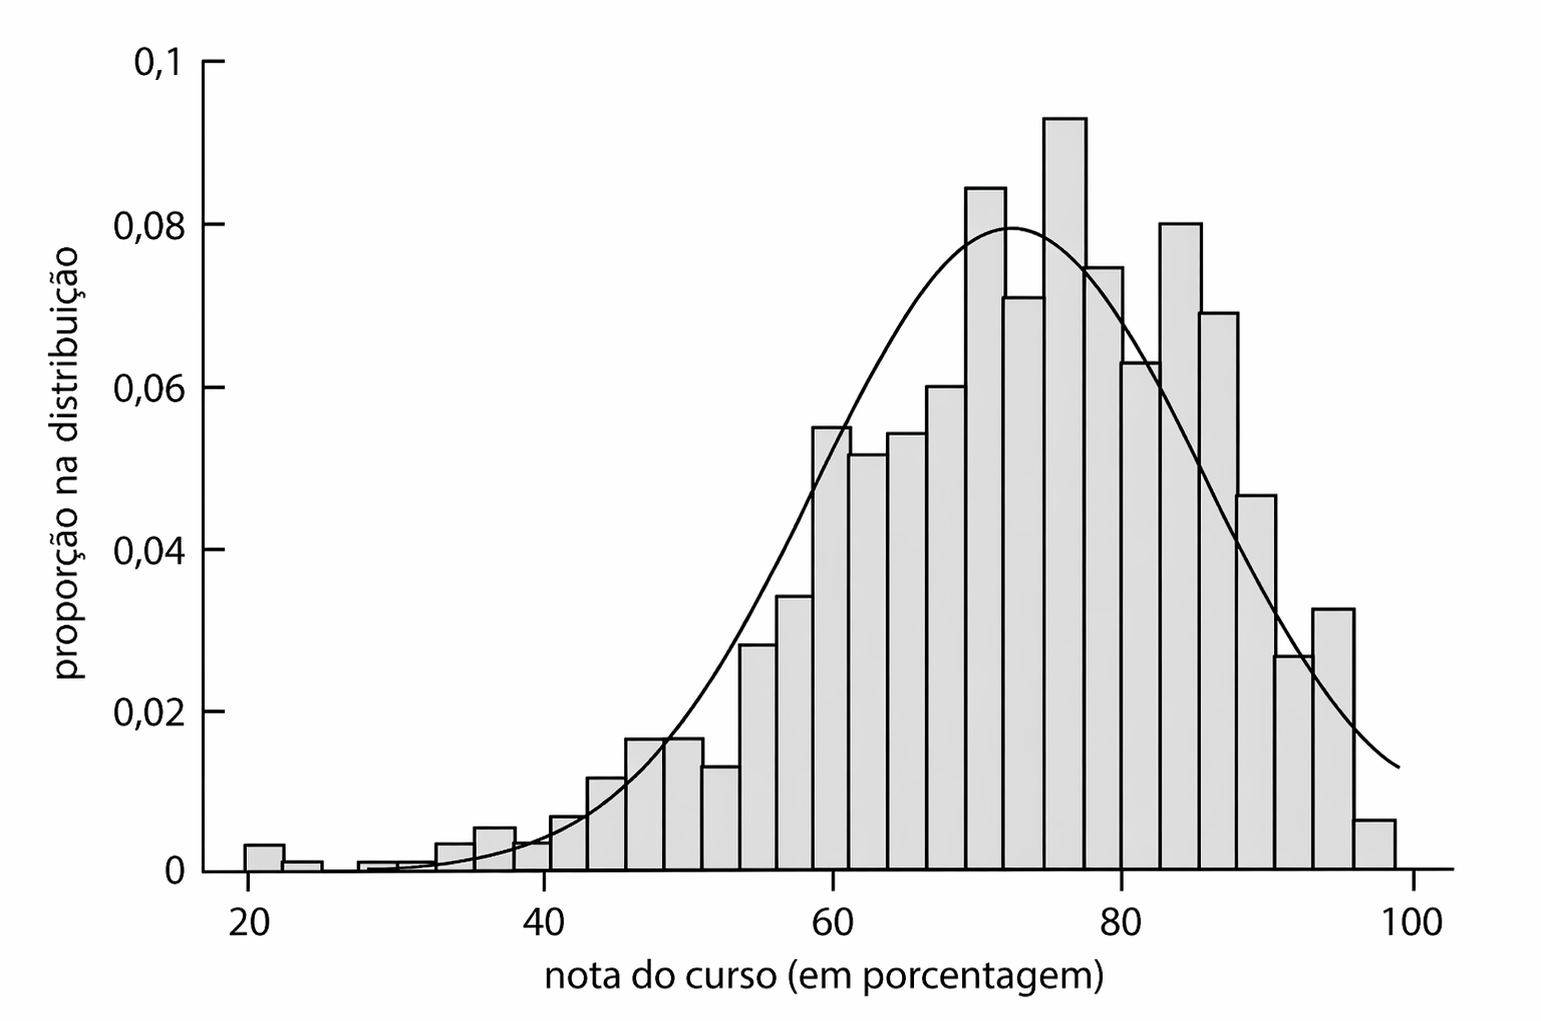
\includegraphics[width=0.75\textwidth]{graph.png}
		\end{center}
		
		\begin{enumerate}[label=(\roman*)]
			\item Se você usar a distribuição normal para estimar a probabilidade de \textit{score} superar 100, a resposta seria zero? Por que sua resposta contradiz a hipótese de uma distribuição normal de \textit{score}?
			
			\item Explique o que está acontecendo na parte esquerda do histograma. A distribuição normal se ajusta bem à parte esquerda do gráfico?
		\end{enumerate}
		
		\question\qstar (6.C9, \citep{wooldridge2016}\footnote{Esta é uma questão computacional. Para instalar o \texttt{R} e o \texttt{RStudio} veja o passo a passo aqui: \href{https://rstudio-education.github.io/hopr/starting.html}{https://rstudio-education.github.io/hopr/starting.html}. Caso tenha dúvidas quanto à linguagem, consulte o material disponibilizado no Moodle, e recomendo também o seguinte material de introdução ao \texttt{R}: \href{https://fhnishida.netlify.app/project/rec2301/sec2/}{https://fhnishida.netlify.app/project/rec2301/sec2/} }. O conjunto de dados \texttt{NBASAL} contém informações salariais e estatísticas carreira de 269 jogadores da National Basketball Association (NBA).
		
		\begin{enumerate}[label=(\roman*)]
			\item Estime um modelo que relacione pontos por jogo (\textit{points}) aos anos na liga (\textit{exper}), \textit{age} e \textit{years} jogando na universidade (\textit{coll}). Inclua um termo quadrático em \textit{exper}; as outras variáveis devem aparecer em nível. Registre os resultados na forma usual.
			
			\item Mantendo os anos na universidade e a idade fixos, por qual valor de experiência o ano seguinte de experiência reduziria os pontos por jogo? Isso faz sentido?
			
			\item Por que você acha que \textit{coll} tem um coeficiente negativo e estatisticamente significativo? (Dica: Jogadores da NBA podem ser convocados antes de terminar suas carreiras universitárias e até mesmo diretamente do Ensino Médio.)
			
			\item Adicione um termo quadrático em \textit{age} à equação. Ele é necessário? O que isso parece sugerir em relação aos efeitos de idade, uma vez que experiência e educação estão controladas?
			
			\item Agora faça a regressão de log(\texttt{wage}) sobre \texttt{points}, \texttt{exper}, \texttt{exper$^2$}, \texttt{age} e \texttt{coll}. Relate os resultados de forma usual.
			
			\item Teste se \texttt{age} e \texttt{coll} são conjuntamente significativos na regressão do item (v). O que isso implica em relação à idade e educação terem efeitos separados sobre salário, uma vez que produtividade e tempo de serviço são levados em conta?
		\end{enumerate}
		
	\end{questions}
	\bibliographystyle{apalike}   % or plainnat, econ, etc.
	\bibliography{refs}
\end{document}
